\documentclass[tikz=true]{standalone}
\usepackage{graphicx, standalone}
\usepackage[compat=1.1.0]{tikz-feynman}
\usepackage{tikz}
\usepackage{amsmath, amssymb}
\usepackage{euler}
\usepackage{fontspec}
\setmainfont{MinionPro}

\renewcommand{\k}{\ensuremath\text{k}}
\newcommand{\kp}{\ensuremath\text{k}'}
\newcommand{\q}{\ensuremath\text{q}}

\renewcommand{\r}{\ensuremath\text{r}}

\newcommand{\ph}{\ensuremath\text{ph}}
\newcommand{\phbar}{\ensuremath\overline{\text{ph}}}
\newcommand{\pp}{\ensuremath\text{pp}}

\newcommand{\dens}{\ensuremath\text{d}}
\newcommand{\magn}{\ensuremath\text{m}}
\newcommand{\sing}{\ensuremath\text{s}}
\newcommand{\trip}{\ensuremath\text{t}}

\renewcommand{\ss}{\ensuremath\sigma\sigma}

\begin{document}

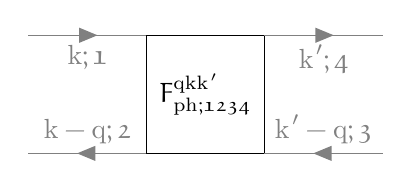
\begin{tikzpicture}[baseline=(current bounding box.center)]
\begin{feynman}
	\vertex (a1);
	\vertex[below=of a1] (a2);
	\vertex[right=of a1] (b1);
	\vertex[below=of b1] (b2);
	\vertex[right=of b1] (c1);
	\vertex[below=of c1] (c2);
	\vertex[right=of c1] (d1);
	\vertex[below=of d1] (d2);

	\node (content) at ($(b1)!0.5!(c2)$) {$F^{\q\k\kp}_{\ph;\mathfrak{1234}}$};	
	
	\diagram* {
		(b1) -- (c1) -- (c2) -- (b2) -- (b1),
		(a1) -- [fermion, gray, edge label'=$\k;\mathfrak{1}$] (b1),
		(b2) -- [fermion, gray, edge label'=$\k-\q;\mathfrak{2}$] (a2),
		(d2) -- [fermion, gray, edge label'=$\k'-\q;\mathfrak{3}$] (c2),
		(c1) -- [fermion, gray, edge label'=$\k';\mathfrak{4}$] (d1),
	};
\end{feynman}
\end{tikzpicture}
\begin{tikzpicture}[baseline=(current bounding box.center)]
	\node {$=$};
\end{tikzpicture}
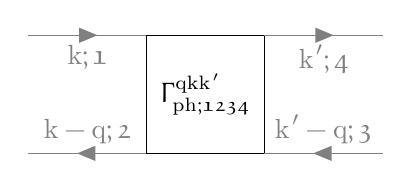
\begin{tikzpicture}[baseline=(current bounding box.center)]
\begin{feynman}
	\vertex (a1);
	\vertex[below=of a1] (a2);
	\vertex[right=of a1] (b1);
	\vertex[below=of b1] (b2);
	\vertex[right=of b1] (c1);
	\vertex[below=of c1] (c2);
	\vertex[right=of c1] (d1);
	\vertex[below=of d1] (d2);

	\node (content) at ($(b1)!0.5!(c2)$) {$\Gamma^{\q\k\kp}_{\ph;\mathfrak{1234}}$};	
	
	\diagram* {
		(b1) -- (c1) -- (c2) -- (b2) -- (b1),
		(a1) -- [fermion, gray, edge label'=$\k;\mathfrak{1}$] (b1),
		(b2) -- [fermion, gray, edge label'=$\k-\q;\mathfrak{2}$] (a2),
		(d2) -- [fermion, gray, edge label'=$\k'-\q;\mathfrak{3}$] (c2),
		(c1) -- [fermion, gray, edge label'=$\k';\mathfrak{4}$] (d1),
	};
\end{feynman}
\end{tikzpicture}
\begin{tikzpicture}[baseline=(current bounding box.center)]
	\node {$+$};
\end{tikzpicture}
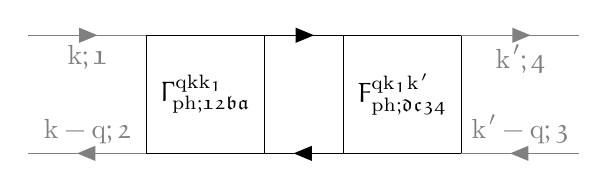
\begin{tikzpicture}[baseline=(current bounding box.center)]
\begin{feynman}
	\vertex (a1);
	\vertex[below=of a1] (a2);
	\vertex[right=of a1] (b1);
	\vertex[below=of b1] (b2);
	\vertex[right=of b1] (c1);
	\vertex[below=of c1] (c2);
	\vertex[right=1cm of c1] (d1);
	\vertex[below=of d1] (d2);
	\vertex[right=of d1] (e1);
	\vertex[below=of e1] (e2);
	\vertex[right=of e1] (f1);
	\vertex[below=of f1] (f2);

	\node (content) at ($(b1)!0.5!(c2)$) {$\Gamma^{\q\k\k_1}_{\ph;\mathfrak{12ba}}$};
	\node (content) at ($(d1)!0.5!(e2)$) {$F^{\q\k_1\kp}_{\ph;\mathfrak{dc34}}$};	
	
	\diagram* {
		(b1) -- (c1) -- (c2) -- (b2) -- (b1),
		(a1) -- [fermion, gray, edge label'=$\k;\mathfrak{1}$] (b1),
		(b2) -- [fermion, gray, edge label'=$\k-\q;\mathfrak{2}$] (a2),
		(d2) -- [fermion] (c2),
		(c1) -- [fermion] (d1),
		(d1) -- (e1) -- (e2) -- (d2) -- (d1),
		(f2) -- [fermion, gray, edge label'=$\kp-\q;\mathfrak{3}$] (e2),
		(e1) -- [fermion, gray, edge label'=$\kp;\mathfrak{4}$] (f1),
	};
\end{feynman}
\end{tikzpicture}

\end{document}